\documentclass{article}


% Packages
\usepackage{fullpage}
\usepackage{amssymb}
\usepackage{multicol}
\usepackage{amsmath}
\usepackage{amsfonts}
\usepackage{bm}
\usepackage{float}
\usepackage{tikz}
\usepackage{xcolor}
\usetikzlibrary{shapes.geometric, positioning, arrows}

% Macros
\newcommand{\R}{\mathbb{R}}
\newcommand{\N}{\mathbb{N}}
\newcommand{\Q}{\mathbb{Q}}
\newcommand{\sub}{\subset}
\renewcommand{\a}{\alpha}
\renewcommand{\b}{\beta}
\newcommand{\ex}{\exists}
\newcommand{\overbar}[1]{\mkern 1.5mu\overline{\mkern-1.5mu#1\mkern-1.5mu}\mkern 1.5mu}

\newtheorem{example}{Example}
\newtheorem{solution}{Solution}
\newtheorem{defintion}{Definition}

\title{The Real Number System}
\author{James Arthur}

\begin{document}
\maketitle
\tableofcontents\newpage

\multicols{2}

\section{Overview}

The reals ($\R$) have a few properties:
\begin{enumerate}
  \item They are a field, i.e. a groupoid with {\color{blue}two binary operations}.
  \item They are ordered
  \item They are also {\color{blue}complete}.
\end{enumerate}
We will also look at {\color{blue}supremum} and the {\color{blue}infimum}.

We are also going to look at the {\color{blue}extended real numbers}. We are going to add two more fictitious points. $\R \cup \{ \infty \} \cup \{ -\infty \}$.

\section{Properties of the Reals}
We will be taking the axiomatic view point of the real numbers. No construction with {\color{blue}Dedekind cuts} or {\color{blue}Cauchy sequences}. All of these are isomorphic.

\subsection{Field Properties}
The real numbers are a set, $\R$, with two binary operations, $+$ and $\times$. They must satisfy the following axioms. So take $a, b, c \in \R$:
\begin{enumerate}
  \item $a + b = b + a$ and $ab = ba$ ({\color{blue}commutativity})
  \item $(a + b) + c = a + (b + c)$ and $a(bc) = (ab)c$ ({\color{blue}associativity})
  \item $a(b + c) = ab + ac$ ({\color{blue}distributivity})
  \item There are two distinctive identities $0$ ({\color{blue}additive identity}) and $1$ ({\color{blue}multiplicative identity}), such that $a + 0 = 0 + a = a$ and $a1 = 1a = a$
  \item We also have inverses, $-a$ ({\color{blue}additive inverse}) such that $a + -a = 0$ and if $a \neq 0$, there is a real number $\frac{1}{a}$ such that: $a(\frac{1}{a})=1$
\end{enumerate}

\subsection{Order Relation}

The real numbers are {\color{blue}ordered}, that means:
\begin{enumerate}
  \item For each pair of reals $a$ and $b$, exactly one of the following is true
  $$ a = b \qquad a < b \qquad b < a $$
  \item It is also {\color{blue}transitive}, if $a < b$ and $b < c$, then $a < c$
  \item If $a < b$ then $a + c < b + c$ for any $c$, and if $0 < c$, then $ac < bc$
\end{enumerate}

\subsection{Supremum}

Let $S\sub \R$. If there exists $b\in\R$ such that $x \le b \quad\forall x\in S$ then $S$ is {\color{blue}bounded above} and $b$ is an {\color{blue}upper bound of $S$}.

If $\b$ is an upper bound of $S$, but no number less than $\b$ is, then $\b$ is called the {\color{blue}supremum} of S, denoted:
$$ \b = \sup S $$
\vspace{-10pt}
\begin{figure}[H]
  \centering
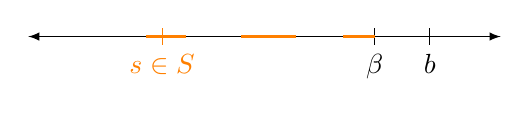
\begin{tikzpicture}
\draw[latex-latex] (-3,0) -- (3,0) ; %edit here for the axis
\draw[shift={(2.1,0)},color=black] (0pt,3pt) -- (0pt,-3pt);
\draw[shift={(2.1,0)},color=black] (0pt,0pt) -- (0pt,-3pt) node[below]
{$b$};
\draw[shift={(1.4,0)},color=black] (0pt,3pt) -- (0pt,-3pt);
\draw[shift={(1.4,0)},color=black] (0pt,0pt) -- (0pt,-3pt) node[below]
{$\b$};
\draw[shift={(-1.3,0)},color=orange] (0pt,3pt) -- (0pt,-3pt);
\draw[shift={(-1.3,0)},color=orange] (0pt,0pt) -- (0pt,-3pt) node[below]
{$s\in S$};
\draw[very thick, color=orange] (1,0) -- (1.4,0);
\draw[very thick, color=orange] (-1.5,0) -- (-1,0);
\draw[very thick, color=orange] (-0.3,0) -- (0.4,0);
\end{tikzpicture}
\caption{\textit{Let $S$ be the orange set and then $b$ is an upper bound of S and $\b$ is $\sup S$}}
\end{figure}
We also call the supremum the least upper bound.\\
\fbox{\parbox{0.475\textwidth}{\begin{example}{
  $S = [\,0, 1\,]$ and prove $sup\, S = 1$
}\end{example}\begin{solution}{
Take our diagram from above:
\begin{figure}[H]
  \centering
\begin{tikzpicture}
\draw[latex-latex] (-3,0) -- (3,0) ; %edit here for the axis
\draw[shift={(0,0)},color=black] (0pt,3pt) -- (0pt,-3pt);
\draw[shift={(0,0)},color=black] (0pt,0pt) -- (0pt,-3pt) node[below]
{$0$};
\draw[shift={(1,0)},color=black] (0pt,3pt) -- (0pt,-3pt);
\draw[shift={(1,0)},color=black] (0pt,0pt) -- (0pt,-3pt) node[below]
{$1$};
\draw[very thick, color=green] (0,0) -- (1,0);
\end{tikzpicture}
\end{figure}
We need to check that $x \le 1 \quad\forall\, x \in S$, which is definitionally true.\\
Secondly we need to prove that $\forall\, b < 1,\: \ex\, x \in S, \,b < x$, which is again trivially true. So $\sup S = 1$
}\end{solution}}}\vspace{10pt}
\fbox{\parbox{0.475\textwidth}{\begin{example}{
 Take $T = (\,0, 1\,)$ where $\sup T = 1$
}\end{example}\begin{solution}{
  Again every number is less than 1, but if you take any number less than one you can always find another element larger.\\
  {\color{red} \textbf{NB: The supremum here isn't in the set}}
}\end{solution}}}\vspace{10pt}

\subsection{Infimum}
Similarly, if there exists an $a \in \R$ such that $a \le x \quad x \in S$, then $S$ is {\color{blue}bounded below} and $a$ is a {\color{blue}lower bound of $S$}.\\

If $\a$ is a lower bound of $S$, but no number is greater than $\a$ is, then $\a$ is called the {\color{blue} infimum } of $S$:
$$ \a = \inf \, S $$
\vspace{-30pt}
\begin{figure}[H]
  \centering
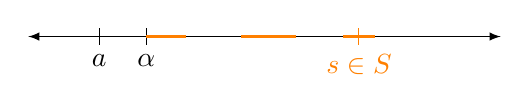
\begin{tikzpicture}
\draw[latex-latex] (-3,0) -- (3,0) ; %edit here for the axis
\draw[shift={(-2.1,0)},color=black] (0pt,3pt) -- (0pt,-3pt);
\draw[shift={(-2.1,0)},color=black] (0pt,0pt) -- (0pt,-3pt) node[below]
{$a$};
\draw[shift={(-1.5,0)},color=black] (0pt,3pt) -- (0pt,-3pt);
\draw[shift={(-1.5,0)},color=black] (0pt,0pt) -- (0pt,-3pt) node[below]
{$\a$};
\draw[shift={(1.2,0)},color=orange] (0pt,3pt) -- (0pt,-3pt);
\draw[shift={(1.2,0)},color=orange] (0pt,0pt) -- (0pt,-3pt) node[below]
{$s\in S$};
\draw[very thick, color=orange] (1,0) -- (1.4,0);
\draw[very thick, color=orange] (-1.5,0) -- (-1,0);
\draw[very thick, color=orange] (-0.3,0) -- (0.4,0);
\end{tikzpicture}
\caption{\textit{Let $S$ be the orange set and then $a$ is a lower bound of S and $\a$ is $\inf\, S$}}
\end{figure}
Another name for the infimum is the greatest lower bound.

\subsection{Completeness Axiom}

Do the supremum and the infimum actually exist? Well, not all subsets are bounded above, i.e. $\R \sub \R$ or what about the empty set? This is what the completeness axiom does:
\begin{enumerate}
  \item If a non-empty set of real numbers are bounded above, then it has a supremum.
\end{enumerate}

So the reals are a {\color{red} \textbf{complete ordered field} }\\

The completeness axiom is distinguishing of the reals. They are the only complete ordered field. The rationals possess everything but completeness in terms of our axioms.\\

\noindent
\fbox{\parbox{0.475\textwidth}{\begin{example}{
 We restrict to the $\Q,\quad S = \{ r \in \Q : r^2 < 2 \} $. Find the supremum and infimum.
}\end{example}\begin{solution}{
If we take the example below;
\begin{figure}[H]
  \centering
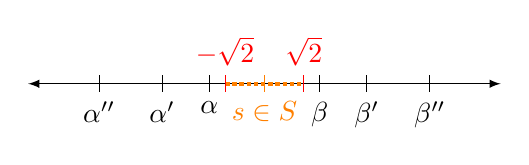
\begin{tikzpicture}
\draw[latex-latex] (-3,0) -- (3,0) ; %edit here for the axis
\draw[densely dotted, ultra thick, orange] (-0.5,0) -- (0.5,0); % adds a dotted line
\draw[shift={(-2.1,0)},color=black] (0pt,3pt) -- (0pt,-3pt);
\draw[shift={(-2.1,0)},color=black] (0pt,0pt) -- (0pt,-3pt) node[below]
{$\a''$};
\draw[shift={(-1.3,0)},color=black] (0pt,3pt) -- (0pt,-3pt);
\draw[shift={(-1.3,0)},color=black] (0pt,0pt) -- (0pt,-3pt) node[below]
{$\a'$};
\draw[shift={(-0.7,0)},color=black] (0pt,3pt) -- (0pt,-3pt);
\draw[shift={(-0.7,0)},color=black] (0pt,0pt) -- (0pt,-3pt) node[below]
{$\a$};
\draw[shift={(2.1,0)},color=black] (0pt,3pt) -- (0pt,-3pt);
\draw[shift={(2.1,0)},color=black] (0pt,0pt) -- (0pt,-3pt) node[below]
{$\b''$};
\draw[shift={(1.3,0)},color=black] (0pt,3pt) -- (0pt,-3pt);
\draw[shift={(1.3,0)},color=black] (0pt,0pt) -- (0pt,-3pt) node[below]
{$\b'$};
\draw[shift={(0.7,0)},color=black] (0pt,3pt) -- (0pt,-3pt);
\draw[shift={(0.7,0)},color=black] (0pt,0pt) -- (0pt,-3pt) node[below]
{$\b$};
\draw[shift={(0,0)},color=orange] (0pt,3pt) -- (0pt,-3pt);
\draw[shift={(0,0)},color=orange] (0pt,0pt) -- (0pt,-3pt) node[below]
{$s\in S$};
\draw[shift={(0.5,0)},color=red] (0pt,3pt) -- (0pt,-3pt);
\draw[shift={(0.5,0)},color=red] (0pt,0pt) -- (0pt,3pt) node[above]
{$\sqrt 2$};
\draw[shift={(-0.5,0)},color=red] (0pt,3pt) -- (0pt,-3pt);
\draw[shift={(-0.5,0)},color=red] (0pt,0pt) -- (0pt,3pt) node[above]
{$-\sqrt 2$};
\end{tikzpicture}
\end{figure}

we can say that we won't reach $\sqrt 2$ in the supremum or $-\sqrt 2$ in the infimum. This is because we are using rationals and $\sqrt 2$ is an irrational. We can go either way and there is always a number closer to $\sqrt 2$.\\

This proves that rationals are not complete.

}\end{solution}}}\vspace{10pt}

\section{Extended Real Numbers}
It is convenient to attach $\infty$ and $-\infty$ to the reals. How do they fit in? Firstly lets look at orders. Take $x\in \R$, then:
$$ -\infty < x <\infty $$
Now if a set $S$ is unbounded above or below, we can write:
$$ \sup\, S =\infty \quad \inf\, S = -\infty $$

\fbox{\parbox{0.475\textwidth}{\begin{example}{
 Find the infimum of $S = \{ x\in \R : x : 2 \}$
}\end{example}\begin{solution}{
\begin{figure}[H]
  \centering
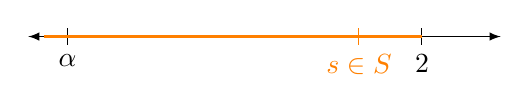
\begin{tikzpicture}
\draw[latex-latex] (-3,0) -- (3,0) ; %edit here for the axis
\draw[shift={(2,0)},color=black] (0pt,3pt) -- (0pt,-3pt);
\draw[shift={(2,0)},color=black] (0pt,0pt) -- (0pt,-3pt) node[below]
{$2$};
\draw[shift={(-2.5,0)},color=black] (0pt,3pt) -- (0pt,-3pt);
\draw[shift={(-2.5,0)},color=black] (0pt,0pt) -- (0pt,-3pt) node[below]
{$\a$};
\draw[shift={(1.2,0)},color=orange] (0pt,3pt) -- (0pt,-3pt);
\draw[shift={(1.2,0)},color=orange] (0pt,0pt) -- (0pt,-3pt) node[below]
{$s\in S$};
\draw[very thick, color=orange] (-2.8,0) -- (2,0);
\end{tikzpicture}
\end{figure}
  As there is technically no lower bound, it is $-\infty$
}\end{solution}}}\vspace{10pt}

We usually denote the extended reals with the symbol, $\overbar{\R} $ or $[-\infty, \infty]$ or $\R \cup \{-\infty, \infty \}$


\subsection{Arithmetic}
If $a \in \R$,
\begin{enumerate}
  \item Then:
  \begin{align*}
    a + \infty &= \infty + a = \infty\\
    a - \infty &= -\infty + a = -\infty\\
    \frac{a}{\infty} &= \frac{a}{-\infty} = 0\\
  \end{align*}
  \item and $0 < a$, then:
  \begin{align*}
    a\infty &= \infty a = \infty \\
    a(-\infty) &= (-\infty)a = -\infty\\
  \end{align*}
  \item and $a < 0$, then:
  \begin{align*}
    a\infty &= \infty a = -\infty\\
    a(-\infty) &= (-\infty)a = \infty\\
  \end{align*}
\end{enumerate}

We also define:
\begin{enumerate}
  \item $\infty + \infty = \infty\infty = (-\infty)(-\infty) = \infty$\\
  \item and also $- \infty - \infty = \infty(-\infty) = (-\infty)\infty = -\infty$\\
  \item and finally, $|\infty| = |-\infty| = \infty$
\end{enumerate}

We say it isn't useful to define; $\infty - \infty$, $0 \cdot \infty$, $\displaystyle{\frac{\infty}{\infty}}$ and $\displaystyle{\frac{0}{0}}$. We call them indeterminate forms.
\end{document}
